\documentclass[12pt,a4paper]{article}

\usepackage[utf8]{inputenc}
\usepackage[ngerman]{babel}
\usepackage[T1]{fontenc}
\usepackage{amsmath}
\usepackage{amsfonts}
\usepackage{amssymb}
\usepackage{graphicx}
\usepackage[left=2cm,right=2cm,top=2cm,bottom=2cm]{geometry}
\usepackage{multicol}
\usepackage{booktabs}
\usepackage[hidelinks]{hyperref}
\usepackage{tikz}
\usepackage{pgfplots}
\usepackage{blindtext}
\usepackage{array}
\usepackage{multirow}
\usepackage{bigdelim}
\usepackage{colortbl}
\usepackage{fancyhdr} 
\usepackage{tabularx}
\usepackage{pgfplots}
\usepackage{xcolor}
\usepackage{color}
\usetikzlibrary{decorations.text}
\usetikzlibrary{tikzmark}
\pagestyle{fancy} 
	\fancyhf{} 
	\fancyhead[L]{
\includegraphics[scale=0.05]{Bilder/dhbw.png}} 
	\fancyhead[C]{\slshape Analysis} 
	\fancyhead[R]{\slshape LaTeX Version}

\usepackage{helvet}
\renewcommand{\familydefault}{\sfdefault}

\newcolumntype{Z}{>{\centering\let\newline\\\arraybackslash\hspace{0pt}}X}
\author{\slshape Robin Rausch, Florian Maslowski, Ozan Akzebe}
\title{Analysis}
\date{\slshape \today}
\begin{document}
\maketitle
\tableofcontents
\newpage
\section{Eigenwerttheorie}
	Der Eigenvektor $\overrightarrow{x} $ ist der Vektor einer Matrix $A$, der sich bei der Multiplikation mit der Matrix
	nur um die Länge mit dem ändert:\\
	\Large $A \cdot \overrightarrow{x} = \lambda \cdot \overrightarrow{x} $\\
	\normalsize sdfs


\section{Quadrik}   
    Die Quadrik ist die Lösungsmenge von quadratischen Gleichungen mit mehreren Variablen.
	
\section{Satz von Bolzano-Weierstrass}
	\begin{enumerate}
		\item Jede beschränkte Folge in $\mathbb{R}$ oder $\mathbb{C}$ hat wenigstens einen Häufungspunkt
  		\item Jede beschränkte Folge in $\mathbb{R}$ oder $\mathbb{C}$ hat wenigstens eine konvergente Teilfolge
	\end{enumerate}


\section{Grenzwert}
	$$\color{red}\text{A ist Grenzwert } \iff \lim_{n\rightarrow\infty}{a_{n}=A} \iff\forall_{\epsilon>0}~\exists_{n_{0}\in\mathbb{N}} ~\forall_{n \leq n_{0}}: | a     		_{n}-A | < \epsilon$$\\
	Für alle Epsilon die Größer als 0 sind, gibt es ein $n_{0}$ $\underline{\text{ab dem}}$ alle Folgenden $n>n_{0}$ Glieder innerhalb des Epsilon-Gürtels liegen. (Das 		heißt $a_{n}$ - Grenzwert ist kleiner 	als Epsilon)\\\\
	Jede Geometrische Folge: $a_{n}=q^{n}$ ist eine Nullfolge, wenn $\color{red}-1<q<1$\\\\
	Geometrische Folgen haben ihre Variablen immer nur als Potenz bsp.: $a_{n}:~\frac{1}{2^{n}}$
	
\section{Cauchykriterium}
	$$\forall_{\epsilon>0}~\exists_{n_{\epsilon}\in\mathbb{N}} ~\forall_{n \geq n_{\epsilon}~, m \geq n_{\epsilon}}: | a_{n}-a_{m} | < \epsilon$$
	Für jedes $\epsilon > 0$ gibt es einen Index $n_{\epsilon} \in \mathbb{N}$, so dass für all $n\geq n_{\epsilon}$ und $m\geq n_{\epsilon}$,\\
	die Abschätzung $| a_{n}-a_{m} | < \epsilon$ erfüllt ist.\\
	Ist das Cauchy kriterium erfüllt ist die Folge konvergent, und hat einen Grenzwert

\section{Konvergenzkriterium}
	$\lim_{n \to \infty} \; a_n = a \Leftrightarrow \forall_{\varepsilon > 0} \exists _{n_\varepsilon \in  \mathbb{N}}$\\
	$\forall_\epsilon > 0, n \in \mathbb{N}\; \exists\; n_\epsilon: n > n_\epsilon \Rightarrow |g-a_n| < \epsilon $
	Für alle positiven Epsilon und natürliche n, gibt es eine Grenze $n_\epsilon $, nach der alle Folgenglieder um weniger als epsilon vom Grenzwert entfernt sind.\\ 

	\subsection{Satz der monotonen Konvergenz}
		Jede noch monoton wachsende/fallende nach oben/unten beschränkte Folge $(a_n)_{n \in \mathbb{N}}$ ist konvergent.\\

	\subsection{Leibniz-Kriterium}
		Wird oft bei alternierenden Folgen angewendet!\newline
		$$\sum^{\infty}_{n=0}{(-1)^k *a_n}$$
		Sei $a_n$ eine monotone, reelle Nullfolge, dann konvergiert die alternierende Reihe

	\subsection{Regel von L'Hospital}
		Für Grenzwerte bei Brüchen, wenn:
		\begin{enumerate}
			\item Zähler und Nenner gegen 0 oder $\pm \infty$ gehen
			\item Grenzwert des Bruchs $\lim_{x \to x_0} \frac{f'(x)}{g'(x)}$ existiert
		\end{enumerate}
		Regel: $\lim_{x \to x_0} \frac{f'(x)}{g'(x)} = \lim_{x \to x_0} \frac{f'(x)}{g'(x)}$

	\subsection{Sandwich-Prinzip}
		Wenn eine Folge zwischen 2 konvergierenden Folgen mit dem selben Grenzwert liegt, konvergiert diese auch gegen den selben Grenzwert.

	\subsection{Wurzel-/Quotientenkriterium}
		Bei Reihen mit Potenzen wird meist das Wurzelkriterium verwendet!\newline
		Quotientenkriterium wird gerne bei Brüchen und Fakultäten verwendet.\newline
		Eine Reihe $ \sum_{}^{} a_k  $ ist absolut konvergent wenn:\\
		$1. \lim_{k \to \infty} \sqrt[k]{|a_k|}  = q < 1$\\
		$2. \lim_{k \to \infty} \frac{|a_{k+1}|}{a_k}  = q < 1$\\
		Wenn $q > 1$ gilt, ist die Reihe divergent.\newline
		Wenn $q = 1$ gilt, kann man keine Aussage über die Konvergenz treffen.


	\subsection{Majoranten-/Minorantenkriterium}
		Das Majotanten- und Minorantenkriterium wird oft bei Reihen folgender Form verwendet:\newline
		$\sum^{\infty}_{k = 1} \frac{P(k)}{Q(k)}$ mit $P$ und $Q$ als Polynomfunktionen!\newline 
		Majorantenkriterium: Die Reihe wird durch eine größere ersetzt, deren Konvergenz bekannt ist.\\
		Minorantenkriterium: Die Reihe wird durch eine kleinere ersetzt, deren Divergenz bekannt ist.

	\subsection{Stetigkeit}
		Eine Funktion ist stetig, falls die Funktion keine Sprünge hat. 
		Linke Seite der Funktion ist gleich rechte Seite der Funktion.\\
		$f(x_0) = \lim_{x \to x_{0^-}} f(x) = \lim_{x \to x_{0^+}} f(x) $ \\
	
	\subsection{Konvergenzradius}
		%Können wir hierzu vlt ein Beispiel einbauen?
		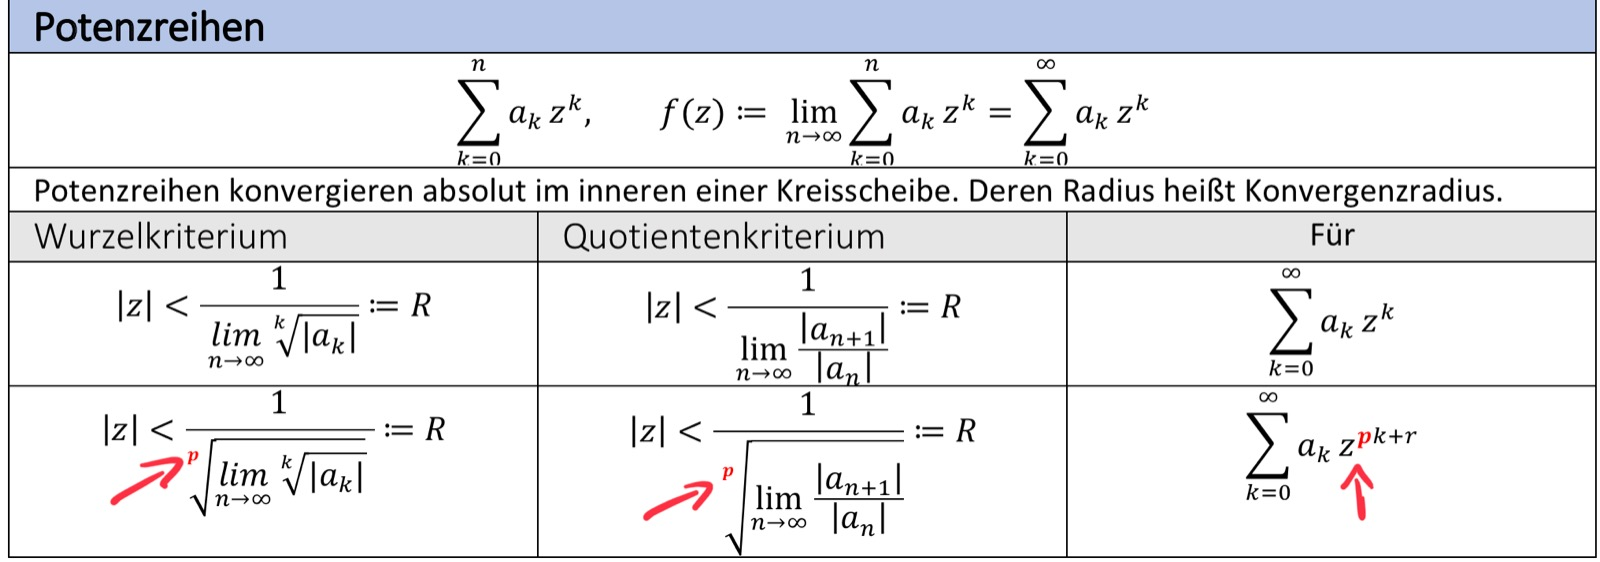
\includegraphics[scale=0.3]{Bilder/Konvergenzradius.jpg}

	\subsection{Wichtigste Potenzreihen}
		$$
		\begin{aligned}
		&\text{Funktion }&& \text{Potenzreihe }&& \text{Bereich} \\
		f(x)&= \frac{1}{1-x}&& =\sum^{\infty}_{n=0}x^{n} && -1 <x <1\\\\
		f(x)&= \ln{(1+x)}&&=\sum^{\infty}_{n=0} \frac{(-1)^{n+1}}{n}*x^{n} && -1 <x <1\\\\
		f(x)&=e^{x} &&= \sum^{\infty}_{n=0}{\frac{1}{n!}}*x^{n}\\\\
		g(x)&=x*e^{x^{2}}&&=x*\sum^{\infty}_{n=0} \frac{{(x^{2})^{n}}}{n!} = \sum^{\infty}_{n=0} \frac{x^{2n+1}}{n!}\\\\
		f(x)&=cos(x) &&= \sum^{\infty}_{n=0}{ \frac{(-1)^{n}}{(2n)!}*x^{2n}}\\\\
		f(x)&=sin(x) &&= \sum^{\infty}_{n=0}{ \frac{(-1)^{n}}{(2n+1)!}*x^{2n+1}}
		\end{aligned}
		$$

\section{Kurvendiskussion}
	\subsection{Newtonverfahren}
		Annähern an Nullstellen durch Rekursion:\\
		$x_{n+1} = x_n - \frac{f(x_n)}{f'(x_n)}$
		
	\subsection{Ableitungen}
		\subsubsection{Grundfunktionen}
			\begin{tabular}{c|c}
				 \hline
				$f(x)$ & $f^{'}(x)$ \\
				\hline
				$x^{n}$ & $n*x^{n-1}$ \\
				\hline\\
				$\frac{1}{x}$ & $- \frac{1}{x^2}$ \\\\
				\hline
				$\sqrt{x}$ & $\frac{1}{2\sqrt{x}}$\\
				\hline
				$e^{x}$ & $e^{x}$ \\
				\hline
				$\ln(x)$ & $\frac{1}{x}$ \\
				\hline
				$\sin{(x)}$ & $\cos{(x)}$ \\
				\hline
				$\cos{(x)}$ & $-\sin{(x)}$ \\
				\hline 
				$\tan{(x)}$ & $\frac{1}{\cos^2(x)}$\\
				\hline 
				$\cot{(x)}$ & $-\frac{1}{\sin^2(x)}$\\
				\hline
				$\sinh{(x)}$ & $\cosh{(x)}$ \\
				\hline
				$\cosh{(x)}$ & $\sinh{(x)}$ \\
				\hline\\
				$\arcsin(x)$ & $\frac{1}{\sqrt{1-x^2}}$\\\\
				\hline\\
				$\arccos(x)$ & $-\frac{1}{\sqrt{1-x^2}}$\\\\
				\hline\\
				$\arctan(x)$ & $\frac{1}{1+x^2}$\\\\
				\hline\\
				arccot$(x)$ & $-\frac{1}{1-x^2}$\\\\
			\end{tabular}\\\\\\
			$\sinh{(x)} = \frac{1}{2}(e^x-e^-x)$ \\\\
			$\cosh{(x)} = \frac{1}{2}(e^x+e^-x)$ 

		\subsubsection{Regeln}
			\begin{tabular}{|c|c|c|}
				 \hline
				Name & Vorher & Nachher \\
				\hline
				Summenregel & $(f\pm g)$ & $f^{'} \pm g^{'}$ \\
				\hline
				Produktregel & $(f*g)$ & $f^{'} *g + f* g^{'}$ \\
				\hline
				Quotientenregel & $(\frac{f}{g})$ & $\frac{f^{'}*g-f*g^{'}}{g^{2}}$ \\
				\hline
				Kettenregel & $f(g(x))$ & $f^{'}(g(x))*g'(x)$ \\
				\hline
			\end{tabular}

	\subsection{Tangentengleichung}
		$$t(x) = f(x_{0}) +f^{'}(x_{0})*(x-x_{0})$$

	\subsection{Stammfunktionen}
		\begin{minipage}[c]{.3\textwidth}
			\begin{tabular}{c|c}
				\hline
			   $f(x)$ & $F(x)$ \\
			   \hline\\
			   $x^{n}$ & $\frac{1}{n+1}x^{n-1}+c$ \\\\
			   \hline\\
			   $\frac{1}{x}$ & $\ln{(|x|)}+c$ \\\\
			   \hline
			   $n*x^{n-1}$ & $x^n + c$\\
			   \hline\\
			   $x$ & $\frac{1}{2}x^2+c$\\\\
			   \hline
			   $2x$ & $x^2+c$\\
			   \hline
			   $\sqrt{x}$ & $\frac{2}{3}x^{\frac{3}{2}} + c$\\
			   \hline\\
			   $\sqrt[n]{x}$ & $\frac{n}{n+1}(\sqrt[n]{x})^{n+1} + c$\\\\
			   \hline
			   $\ln{x}$ & $x*\ln{(x)} -x + c$\\
			   \hline
			   $e^x$ & $e^x + c$\\
			   \hline\\
			   $e^{z*x}$ & $\frac{1}{z}e^{z*x} + c$\\\\
			   \hline
			   $\sin{(x)}$ & $-\cos{(x)}+ c$\\
			   \hline
			   $\cos{(x)}$ & $sin{(x)} + c$\\
		   \end{tabular}
		\end{minipage}
		\begin{minipage}[c]{0.7\textwidth}
			\begin{center}
				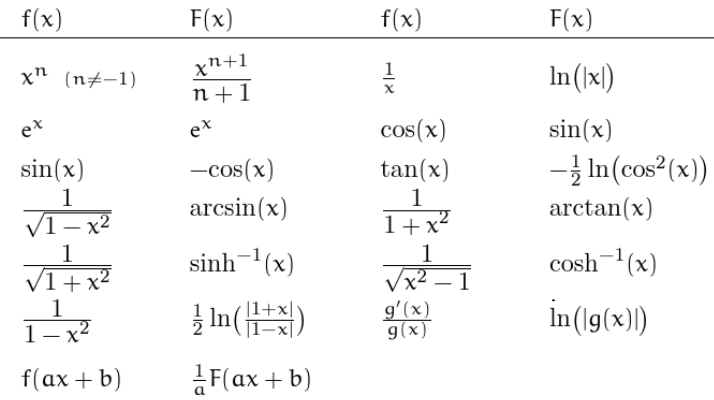
\includegraphics[scale=0.8]{Bilder/Stammfunktionen.PNG}
			\end{center}
		\end{minipage}
			

	\subsection{Definitionsbereich und Wertemenge bestimmen}
		Definitionsberich: Was darf man alles für x einsetzen darf. \\
		Wertemenge: Die Menge die rauskommt, wenn man alles aus der Definitionsmegne einsetzt

	\subsection{Nullstellen berechenn}
		Gleichung gleich 0 setzen (f(x) = 0) und ausrechnen

	\subsection{Y-Achsenabschnitt}
		In die Funktion x=0 einsetzen und das Ergebnis berechnen

	\subsection{Symmetrieverhalten bestimmen}
		\subsubsection{Achsensymmetrie zur y-Achse}
			Prüft, ob bei $f(-x)=f(x)$ dasselbe rauskommt
		\subsubsection{Punktsymmetrie}
			Punktsymmetrie liegt vor, wenn $-f(x)=f(-x)$

	\subsection{Extremstellen/werte und Hoch/Tiefpunkte berechnen}
		Extremstellen: $f^{'}(x) = 0$\\
		Hoch- oder Tiefpunkt: $f^{''}(x)$ an der Nullstelle von $f^{'}(x)$ 
			Ist $f^{''}(x)>0$ Tiefpunkt
			Ist $f^{''}(x)<0$ Hochpunkt

	\subsection{Wendepunkt}
		2. Ableitung bestimmen und Nullstellen berechnen $\rightarrow$ hier sind Wendepunkte
		3. Ableitung bestimmen um zu bestimmen, ob Rechts-Links-Wendepunkt oder Links-Rechts Wendepunkt 
			$f^{'''}(x)>0$ rechts-links gekrümmt 
			$f^{'''}(x)<0$ links-rechts gekrümmt
			$f^{'''}(x)=0$ kein Wendepunkt

\section{Taylor Entwicklung}
	Taylor Reihen sind Annäherungen an Funktionen um einen Punkt x an der Funktion. Hierzu wird die Funktion solange abgeleitet, bis ein Muster zu erkennen ist und dieses dann zu einer Reihe(mit Summenzeichen) umgeformt werden kann.\\ 
	Formel: $f(x) = \sum_{i = 0}^{\infty} \frac{f^{(i)}(x_0)}{i!} \cdot (x-x_0)^i$\newline
	\newline
	\textbf{Wichtige Taylorreihen sind zum Beispiel:}\newline
	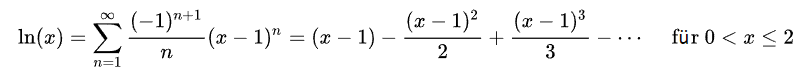
\includegraphics[]{Bilder/ln_von_x_taylor.PNG}\newline
	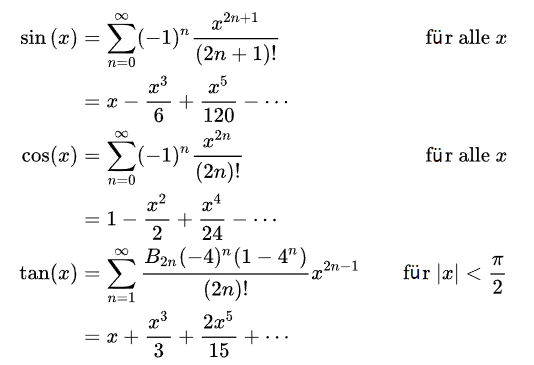
\includegraphics[scale=1.2]{Bilder/trigonometrische_taylor.PNG}\newline
	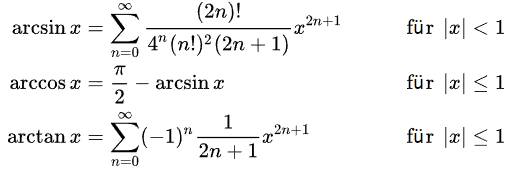
\includegraphics[scale=1.2]{Bilder/mehr_trigonometrische_taylor.PNG}

\section{Integrale}
	\subsection{Berechnung}
		$\int^a_b{f(x)} = F(a) - F(a)$

	\subsection{Integralregeln}
		\begin{enumerate}
			\item Faktorregel \\
				$\int {c*f(x)dx} = c * \int {f(x)dx}$
			\item Potenzregel\\
				$\int{x^n}dx = \frac{x^{n+1}}{n+1}$   $, x \ne -1$
			\item Summenregel \\
				$\int {(f(x) + g(x))dx} = \int{f(x)dx} + \int{g(x)dx}$ 
			\item Partielle Integration\\
				$\int{f(x)*g^{'}(x)dx} = f(x)*g(x) - \int{f^{'}(x)*g(x)dx}$
			\item Substitutionsregel \\ 
				$\int{f(g(x)) * g^{'}(x)dx} =\int{f(g(x))dx}$
			\item Logarithmische Integration\\
				$\int{\frac{f^{'}(x)}{f(x)}dx} = \ln{(|f(x)|)} $
			\item Vertauschungsregel \\
				$\int^a_b{f(x)dx} = - \int^b_a{f(x)dx}$
			\item Gleichheit von oberer und unterer Grenze \\
				$\int^a_a{f(x)dx} = 0$
		\end{enumerate}
		
		\subsubsection{Substitutionsregel Beispiel}
		\textbf{Beispiel 1:}\newline
		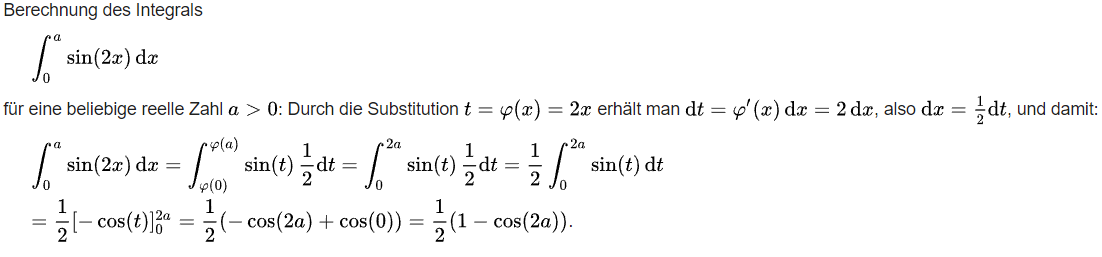
\includegraphics[scale=0.85]{Bilder/substitutionsregel1.PNG}\newline
		\textbf{Beispiel 2:}\newline
		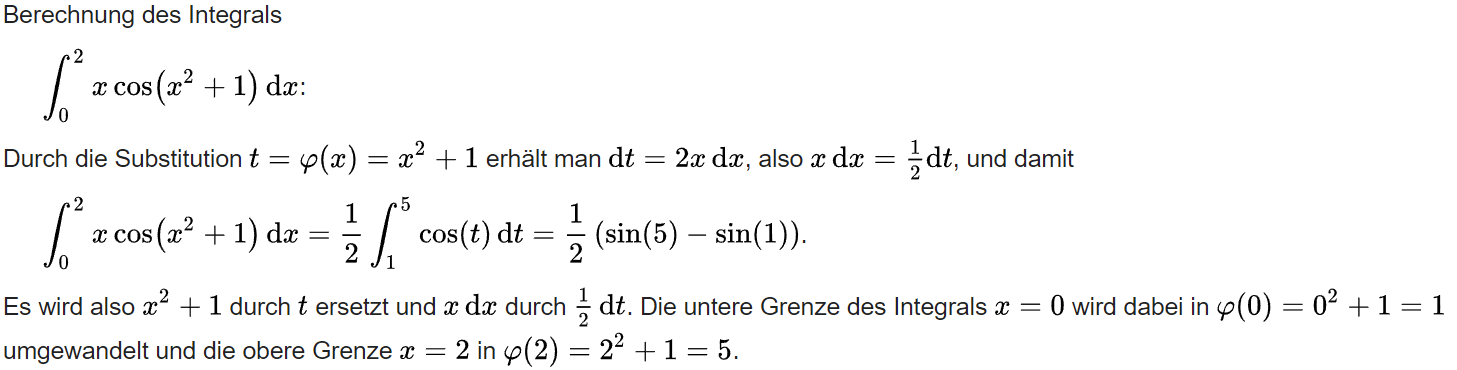
\includegraphics[scale=0.65]{Bilder/substitutionsregel2.PNG}
	
	\subsection{Patrielle Integration}
	\begin{center}
		$\int u \cdot v' \,dx = u \cdot v - \int u' \cdot v \,dx$
	\end{center}
	bzw.\newline
	\begin{center}
		$\int u(x) \cdot v'(x) \,dx = u(x) \cdot v(x) - \int u'(x) \cdot v(x) \,dx$
	\end{center}
	Hierbei ist es leichter wenn u (bzw. u(x)) der durch Ableiten \textit{leichter} werdende Term ist. Also z.B. $2x^2$ oder $x$. \newline
	Das v' (bzw. v'(x)) ist dann der sich weniger verändernde Teil. Also z.B. $e^x$

\end{document}